\documentclass[manual-fr.tex]{subfiles}
\begin{document}

Une fois les fichiers d'entraînement et la chaîne de traitements sélectionnés, cliquer sur le bouton «~train SEM~» comme illustré dans la figure \ref{fig:train_sem-03}. Cela ouvrira la fenêtre qui vous permettra de paramétrer le CRF pour réapprendre SEM, illustrée dans la figure \ref{fig:train_sem-03}. Dans cette fenêtre, vous avez notamment la possibilité de choisir un fichier pattern pour Wapiti. Si vous n'en choisissez pas, il sera automatiquement généré depuis les traits générés par la chaîne de traitement. Lorsque tous les paramètres sont configurés, cliquer sur le bouton «~train~» pour lancer l'entraînement d'un nouveau modèle de SEM. Lorsque l'entraînement sera terminé, SEM indiquera où vous aurez la possibilité de récupérer les fichiers, comme illustré dans la figure \ref{fig:train_sem-06}. Pour pouvoir utiliser le modèle, il faut copier le fichier «~model.txt~» dans le dossier «~\$\{SEM\_DATA\}/resources/models/fr/NER~».

\begin{figure}[ht!]
    \begin{center}
    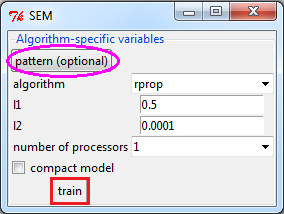
\includegraphics[scale=0.75]{fr/images/train_sem-05.png}
    \end{center}
    \caption{Entouré en violet : le bouton pour sélectionner un modèle particulier. Encadré en rouge : le bouton pour lancer l'entraînement.}
    \label{fig:train_sem-05}
\end{figure}

\begin{figure}[ht!]
    \begin{center}
    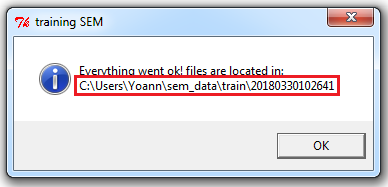
\includegraphics[scale=0.75]{fr/images/train_sem-06.png}
    \end{center}
    \caption{Encadré en rouge : le chemin où trouver le fichier enregistré}
    \label{fig:train_sem-06}
\end{figure}

\end{document}
